%==============================================================================
\chapter{Methodik}
\label{chap:methodik}
%==============================================================================
Ziel dieser Arbeit ist die Entwicklung einer Methode für die Modellierung von Kraftstoffsystemen von Fluggasturbinen für Schmalrumpfflugzeuge, um deren Auslegung zu unterstützen. Insbesondere wird angestrebt, eine Vergleichbarkeit des Wärme-/Leistungsbedarfs zwischen kerosinbetriebenen und wasserstoffbetriebenen Kraftstoffsystemen zu ermöglichen. 

Hierfür wird zunächst das mathematische Problem der Kraftstoffsysteme formuliert und die Lösung beschrieben. Anschließend wird  das CFM56-5B Triebwerk als Referenzarchitektur nachgebildet und es werden denkbare Architekturen für wasserstoffbetriebene Kraftstoffsysteme erarbeitet. Im nächsten Schritt werden die für die Modellierung der Kraftstoffsysteme notwendigen Komponentenmodelle entwickelt. Abschließend werden die verwendeten Stoffmodelle für die beiden Kraftstoffe beschrieben und sämtliche für die Modellierungen notwendigen Parameter ermittelt.

\section{Annahmen und Vereinfachungen}

Um einen Kompromiss zwischen Detailtiefe, Genauigkeit und Rechenaufwand zu finden, werden in dieser Arbeit mehrere Vereinfachungen verwendet. Insbesondere gelten die betrachteten Modelle lediglich für den stationären Fall. Da der Fokus dieser Arbeit auf der Vorauslegungsrechnung liegt, werden transientes Systemverhalten sowie Off-Design-Verhalten nicht betrachtet. 

Zudem wird in den für die Modellierung relevanten Querschnitten der Kraftstoffsysteme von vernachlässigbaren Geschwindigkeiten, beziehungsweise kinetischen Energien ausgegangen. Innerhalb der modellierten Turbomaschinen ist diese Annahme nicht gültig, jedoch beschränkt sich die Modellierung auf die Erfassung der Größen in den Leitungen zwischen den jeweiligen Komponenten. Bei einer konservativ abgeschätzten Machzahl in den Leitungen $Ma_L=0.1$ und mit dem Isentropenexponenten $\kappa_{\mathrm{H}_2} = 1.4$ beträgt das mit der Isentropenbeziehung berechnete total zu statische Temperaturverhältnis  $\frac{T_{t,L}}{T_L}$

\begin{equation}\label{Eq:mach}
	\frac{T_{t,\mathrm{L}}}{T_\mathrm{L}}=1+\frac{\kappa_{\mathrm{H}_2}-1}{2}Ma_\mathrm{L}^2
\end{equation}

lediglich $1,002$. Unter Annahme eines maximalen Wasserstoffmassenstroms von \SI{0.731}{\kg\per\s} bei einer Temperatur von \SI{300}{\K} beträgt der maximale Leitungsdurchmesser \SI{69}{\milli\m}, was als unkritisch eingestuft wird.

\section{Mathematische Formulierung}

Die Modellierung der Kraftstoffsysteme kann vereinfacht als Funktion $f$ betrachtet werden, welche die unabhängigen Variablen $x$ (Pumpenleistungen, Wärmezufuhr etc.) mithilfe der bekannten Parameter $P$ (Wirkungsgrade, Randbedingungen etc.) auf die abhängigen Variablen $y$ (z.B. Brennkammer-Eintrittstemperatur)

\begin{equation}\label{Eq:fuel_func}
	y = f(x, P)
\end{equation}

abbildet. Zu den Parametern $P$ zählen hierbei beispielsweise als konstant angenommene Pumpenwirkungsgrade und der Ausgangszustand der Kraftstoffe. Für den Zweck dieser Betrachtung fallen unter die unabhängigen Variablen Größen wie der Austrittsdruck der Hochdruckpumpe. Der Brennkammer-Eintrittsdruck und die Brennkammer-Eintrittstemperatur sind Beispiele für die abhängigen Variablen. Für den Zweck dieser Arbeit ist allerdings von Interesse, inwiefern sich die abhängigen Variablen die unabhängigen Variablen auswirken. So ist eine relevante Fragestellung, welche Wärmezufuhr zum erreichen einer bestimmten Brennkammer-Eintrittstemperatur erforderlich ist. Mathematisch entspricht dies der Umkehrfunktion $f^{-1}$, welche die abhängigen Variablen $y$ auf die unabhängigen Variablen $x$

\begin{equation}\label{Eq:fuel_inverse}
	x = f^{-1}(y, P)
\end{equation}

abbildet. Eine analytische Herleitung der Umkehrfunktion der Modellierungen der Kraftstoffsysteme zu bilden, ist nicht möglich. Es ist daher notwendig die Werte der Umkehrfunktion numerisch zu approximieren. Der Lösungsansatz dieser Arbeit für dieses mathematische Problem ist in Abbildung \ref{fig:solver} dargestellt. 

\begin{figure}[ht]
\centering
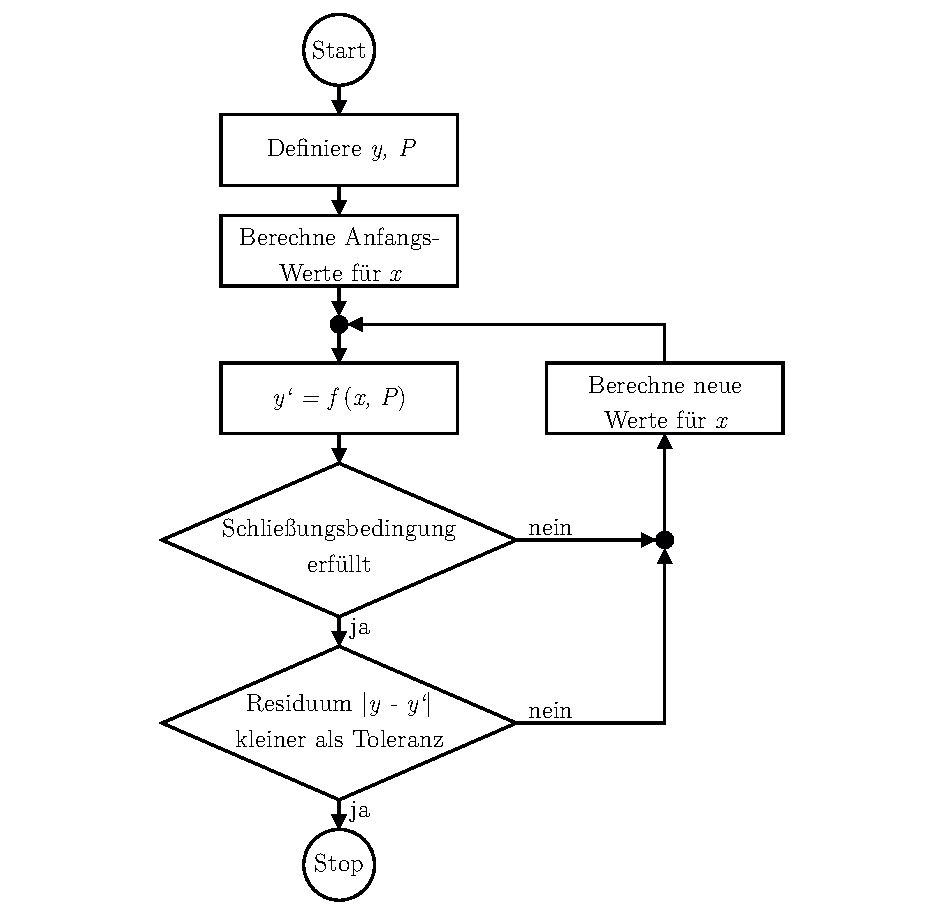
\includegraphics[width=0.8\linewidth]{4_Abbildungen/2_Hauptteil/solver.pdf}
  \caption{Numerische Berechnung von Werten der Umkehrfunktion}
  \label{fig:solver}
\end{figure}
\FloatBarrier 

Zunächst werden die Parameter und die Zielwerte für die abhängigen Variablen definiert. Mithilfe der Zielwerte werden vernünftige Startwerte für die unabhängigen Variablen geschätzt. An dieser Stelle beginnt die iterative Lösung der Modellierung. In jeder Iteration wird mit den gegebenen Werten der unabhängigen Variablen ein Wert für die abhängigen Variablen $y'$ berechnet. Wenn das Residuum, also der Betrag der Differenz zwischen dem Zielwert und dem  berechneten Wert der abhängigen Variable, die Toleranz unterschreitet, ist die Lösung erfolgreich abgeschlossen. Die spezifische Enthalpie der rezirkulierten Kraftstoffmassenströme in dem vorwärts-rechnenden Modell ist unbekannt. Es wird daher mit dem Wert der vorherigen Iteration gerechnet. Dieser Umstand wird durch Einführung einer Schließungsbedingung berücksichtigt. Die Bedingung gilt als erfüllt, wenn der Betrag der Differenz der spezifischen Enthalpien der letzten zwei Iterationen einen geringeren Wert als die Toleranz erreicht.

\section{Referenz-Kraftstoffsystem}

Als Referenzkraftstoffsystem für kerosinbetriebene Triebwerke wird das Kraftstoffsystem des CFM56-5B Triebwerks herangezogen. Die Kraftstoffsysteme der Triebwerke der jüngsten Generation, wie beispielsweise des Pratt \& Whitney PW1133G, sind in der vorhandenen Sachliteratur noch nicht ausführlich dokumentiert. Das andere in der Airbus A320ceo Familie eingesetzte Triebwerk, das IAE V2500-A5 Triebwerk, stellt eine denkbare Alternative dar. Das IAE V2500-A5 ist jedoch nicht gut für die Zwecke einer Modellierung im Rahmen dieser Arbeit geeignet, da das Kraftstoffrückführventil des  Triebwerks Funktionen aufweist, die in der verfügbaren Literatur nicht ausreichend beschrieben sind \cite{LinkeDiesinger.2014}. Als verbleibendes Triebwerk der Airbus A320ceo Familie fällt die Wahl daher auf das CFM56-5B Triebwerk. 

\subsection{Systemarchitektur}

Die Modellierung des Referenzkraftstoffsystems orientiert sich an der vereinfachten Darstellung des Kraftstoffsystems des CFM56-5B Triebwerks in Kapitel \ref{chap:grundlagen}. Eine schematische Darstellung der Modellierung des Referenzkraftstoffsystems ist in Abbildung \ref{fig:Referenz} gegeben.

\begin{figure}[ht]
\centering
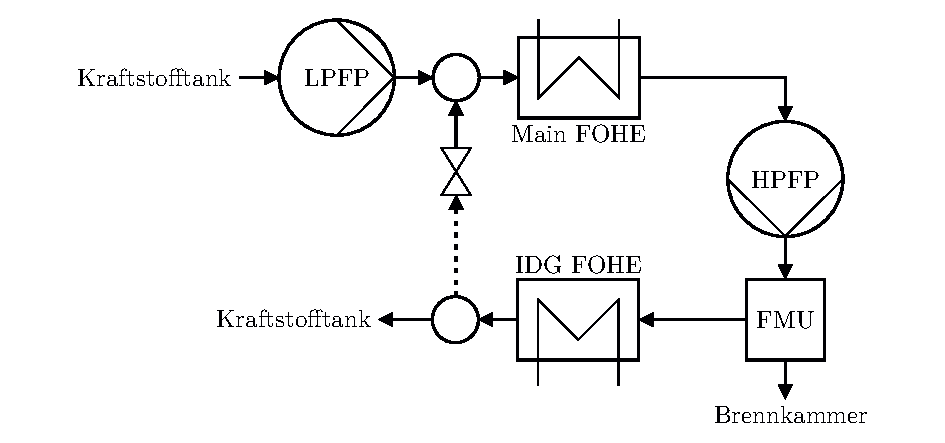
\includegraphics[width=1\linewidth]{4_Abbildungen/2_Hauptteil/Kraftstoffsystem Abbildungen/Referenz.pdf}
  \caption{Referenzkraftstoffsystem}
  \label{fig:Referenz}
\end{figure}
\FloatBarrier 

In dieser Arbeit werden nur Komponenten, die sich innerhalb der Triebwerksgondel befinden, betrachtet. Die Kraftstofftanks und die darin befindlichen Boosterpumpen werden daher nicht modelliert. In der Modellierung wird stattdessen eine Versorgung der Niederdruckpumpe mit dem benötigten Kraftstoffmassenstrom, bei  konstanten Eintrittsbedingungen $T_0, p_0$ angenommen. 

Die Niederdruckpumpe pumpt den Kraftstoff auf einen Austrittsdruck $p_{\mathrm{LPFP}}$ mit einem isentropen Wirkungsgrad $\eta_{\mathrm{LPFP}}$ und einer Leistung $P_{LPFP}$. Da die Modellierung vorwärts rechnet, ist es nicht möglich die spezifische Enthalpie $h_\mathrm{R}$ des rezirkulierten Kraftstoffs direkt innerhalb derselben Iteration zu integrieren. Stattdessen wird die in der vorherigen Iteration berechnete spezifische Enthalpie des rezirkulierten Kraftstoffmassenstroms verwendet. Der rezirkulierte Kraftstoffmassenstrom $\dot{m}_\mathrm{R}$ wird so gewählt, dass die Brennkammer-Eintrittstemperatur $T_{\mathrm{BK}}$ eingehalten wird. 

Der gemischte Kraftstoffmassenstrom durchläuft anschließend den Wärmeübertrager für das Hauptölsystem, nimmt dabei die Wärme $\dot{Q}_{\mathrm{FOHE}}$ auf und erleidet Druckverluste mit dem Druckverhältnis $\pi_{\mathrm{FOHE}}$. Der erwärmte Kraftstoffmassenstrom wird nun in der Hochdruckpumpe mit dem isentropen Wirkungsgrad $\eta_{\mathrm{HPFP}}$ und einer Leistung $P_{\mathrm{HPFP}}$ gepumpt. Der Austrittsdruck der Hochdruckpumpe $p_{\mathrm{HPFP}}$ wird so gewählt, dass der Brennkammer-Eintrittsdruck $p_{\mathrm{BK}}$ erreicht wird. Die Hochdruckpumpe ist als Zahnradpumpe ausgeführt. Da die Hochdruckpumpe für den maximalen Kraftstoffverbrauch im Startfall dimensioniert wird, ist der geförderte Massenstrom im Reiseflug $\dot{m}_{\mathrm{HPFP}}$ vorgegeben. 

Vor dem Eintritt in die Kraftstoffregeleinheit werden in den Leitungen des Kraftstoffsystems auftretende Druckverluste $\Delta p_{\mathrm{L}}$  berücksichtigt. In der Kraftstoffregeleinheit wird der Kraftstoffmassenstrom für die Versorgung der Brennkammer $\dot{m}_{\mathrm{BK}}$ abgezweigt. In den Injektoren erfährt der Kraftstoff den Druckverlust $\Delta p_{\mathrm{inj}}$. 

Der übrige Kraftstoff durchläuft den Wärmeübertrager für das Ölsystem des Stromgenerators und nimmt dabei die Wärme $\dot{Q}_{\mathrm{IDG}}$ auf. Da der rezirkulierte Kraftstoff anschließend gedrosselt wird, wirken sich die Druckverluste dieses Wärmeübertragers nicht auf die Modellierung aus. Nachdem der letzte Wärmeübertrager durchlaufen wurde, wird die spezifische Enthalpie des rezirkulierten Massenstroms berechnet.

\subsection{Variablen und Parameter}

Die abhängigen Variablen des Referenzkraftstoffsystems sind der Brennkammer-Eintrittsdruck $p_{\mathrm{BK}}$ und die Brennkammer-Eintrittstemperatur $T_{\mathrm{BK}}$. Tabelle \ref{Tab:referenz_params} zeigt die Parameter und unabhängigen Variablen des Referenzkraftstoffsystems.

\begin{table}[ht]
    \centering
	\caption{Parameter und Variablen der Modellierung des  Referenzkraftstoffsystems}
	\begin{tabular} {|l|c|l|c|} \hline%
		\multicolumn{2}{|c}{Parameter} & \multicolumn{2}{|c|}{unabhängige Variablen}\\ \hline\hline%
        LPFP-Eintrittstemperatur & $T_0$ & HPFP-Austrittsdruck & $p_{\mathrm{HPFP}}$ \\ \hline
        LPFP-Eintrittsdruck & $p_0$ & HPFP-Leistung & $P_{\mathrm{HPFP}}$ \\ \hline
        FOHE-Wärme & $\dot{Q}_{\mathrm{FOHE}}$ & LPFP-Leistung & $P_{\mathrm{LPFP}}$ \\ \hline
        FOHE-Druckverhältnis & $\pi_{\mathrm{FOHE}}$ & rezirkulierter Massenstrom & $\dot{m}_\mathrm{R}$ \\ \hline
        IDG-FOHE-Wärme  & $\dot{Q}_{\mathrm{IDG}}$ & spezifische Enthalpie von $\dot{m}_\mathrm{R}$ & $h_\mathrm{R}$                 \\ \hline
        LPFP-Austrittsdruck & $p_{\mathrm{LPFP}}$& \multicolumn{2}{c|}{}\\ \hline
        isentroper Wirkungsgrad LPFP & $\eta_{\mathrm{LPFP}}$& \multicolumn{2}{c|}{}\\ \hline
        isentroper Wirkungsgrad HPFP & $\eta_{\mathrm{HPFP}}$& \multicolumn{2}{c|}{}\\ \hline
        HPFP-Massenstrom & $\dot{m}_{\mathrm{HPFP}}$& \multicolumn{2}{c|}{}\\ \hline
        Brennkammermassenstrom & $\dot{m}_{\mathrm{BK},0}$& \multicolumn{2}{c|}{}\\ \hline
        Leitungsdruckverluste & $\Delta p_{\mathrm{L}}$& \multicolumn{2}{c|}{}\\ \hline
        Injektordruckverluste & $\Delta p_{\mathrm{inj}}$& \multicolumn{2}{c|}{}\\ \hline
	\end{tabular}	
    \label{Tab:referenz_params}%
\end{table}
\FloatBarrier 

\section{Wasserstoff-Kraftstoffsystemarchitekturen}

Im folgenden werden unterschiedliche Architekturen für Wasserstoff-Kraftstoffsysteme ausgearbeitet und beschrieben. Abschließend werden die für die Modellierung der Architekturen notwendigen Parameter erläutert. 

Bei den Wasserstoff-Kraftstoffsystemen werden insbesondere zwischen Systemen mit Hochdruckpumpe und Hochdruckverdichter unterschieden. Die Hochdruckpumpe hat den Vorteil eines geringen Leistungsbedarfs, jedoch birgt die Pumpe aufgrund der aufwendigen Schmierung ein höheres Technologierisiko. 

Insgesamt werden drei unterschiedliche Kraftstoffsystemarchitekturen betrachtet. Neben einem Kraftstoffsystem mit Hochdruckpumpe werden zwei Systeme mit Verdichter betrachtet. Die beiden Systeme mit Verdichter unterscheiden sich darin, wie sie den Wasserstoff verdampfen. Bei dem Kraftstoffsystem mit Verdampfer wird der Wasserstoff in einem Wärmeübertrager mit Kraftstoff aus dem Hochdrucksystem verdampft. Bei dem Kraftstoffsystem mit Vormischung wird eine geringe Menge Wasserstoff aus dem Hochdrucksystem vor den Verdichter rezirkuliert, um den Kraftstoff vollständig zu verdampfen.

\subsection{Architektur mit Hochdruckpumpe}

Im Gegensatz zu dem konventionellen Kraftstoffsystem wird bei der Wasserstoff-Kraftstoffsystemarchitektur mit Hochdruckpumpe die Funktion der Pumpe nicht auf eine Hochdruck- und eine Niederdruckpumpe mit Wärmeübertragern dazwischen aufgeteilt. Eine Wärmezufuhr hinter einer möglichen Niederdruckpumpe würde den Wasserstoff schon vor der Hochdruckpumpe verdampfen. Die Lösung besteht darin, den Wasserstoff mit einer einzelnen Kreiselpumpe direkt in das Hochdrucksystem zu pumpen und erst daraufhin Wärme zuzuführen. Die hier diskutierte Kraftstoffsystemarchitektur basiert auf einem von Brewer diskutierten Kraftstoffsystem \cite{Brewer.1991}, jedoch wurden keine Wärmeübertrager mit der Turbinenkühlluft und dem Turbinenabgas vorgesehen. Stattdessen versorgt eine parallele Wasserstoffverbrennung den auftretenden Wärmefehlbetrag zwischen dem Bedarf und der verfügbaren Abwärme. Das Wasserstoff-Kraftstoffsystem mit Pumpe ist in  Abbildung \ref{fig:pumpe} dargestellt.

\begin{figure}[ht]
\centering
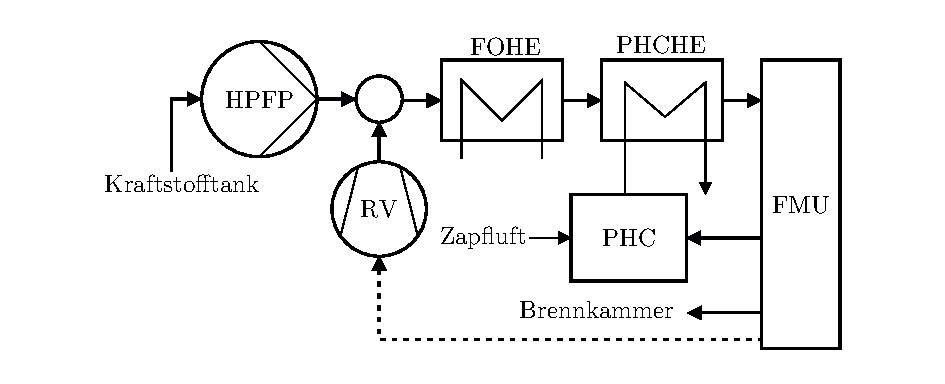
\includegraphics[width=1\linewidth]{4_Abbildungen/2_Hauptteil/Kraftstoffsystem Abbildungen/pump.pdf}
  \caption{Wasserstoffkraftstoffsystem mit Pumpe adaptiert aus \cite{Brewer.1991}}
  \label{fig:pumpe}
\end{figure}
\FloatBarrier 

Der Wasserstoff erreicht das Triebwerk im flüssigen Zustand mit dem Eintrittsdruck $p_0$ und der Eintrittstemperatur $T_0$ und wird direkt in der Hochdruckpumpe auf den Druck $p_{\mathrm{HPFP}}$ gepumpt, sodass der Brennkammer-Eintrittsdruck $p_{\mathrm{BK}}$ erreicht wird. Die Hochdruckpumpe arbeitet mit dem isentropen Wirkungsgrad $\eta_{\mathrm{HPFP}}$ und benötigt die Leistung $P_{\mathrm{HPFP}}$. 

Im Anschluss an die Hochdruckpumpe wird der Kraftstoffmassenstrom $\dot{m}_\mathrm{R}$ mit der spezifischen Enthalpie $h_\mathrm{R}$ dazugemischt. Der warme rezirkulierte Kraftstoff verdampft den flüssigen Kraftstoff und erwärmt diesen auf die Wärmeübertrager-Eintrittstemperatur $T_\mathrm{W}$, um Vereisungen im Ölsystem zu vermeiden.

Auf den Wärmeübertrager mit dem Klimasystem, folgt der Wärmeübertrager mit dem Ölsystem. Der Einfachheit halber werden die beiden Wärmeübertrager in der Modellierung zusammengefasst. In den beiden Wärmeübertragern wird dem Kraftstoff in Summe die Wärme $\dot{Q}_{\mathrm{FOHE}}$ zugeführt. Über die beiden Wärmeübertrager liegt das Druckverhältnis $\pi_{\mathrm{FOHE}}$ vor. Der durch den Wärmeübertrager mit dem Klimasystem gesparte Fan-Zapfluftbedarf wird in der Modellierung nicht berücksichtigt. Um die angestrebte Brennkammer-Eintrittstemperatur $T_{\mathrm{BK}}$ zu erreichen, wird durch eine parallele Wasserstoffverbrennung (engl.: Parallel Hydrogen Combustion, PHC) in einem weiteren Wärmeübertrager (engl.: PHC Heat Exchanger, PHCHE) die zusätzliche Wärme $\dot{Q}_{\mathrm{PHC}}$ zugeführt. Dieser Wärmeübertrager verursacht das Druckverhältnis $\pi_{\mathrm{PHC}}$. 

Vor dem Eintritt in die Kraftstoffregeleinheit werden in den Leitungen des Kraftstoffsystems auftretende Druckverluste $\Delta p_\mathrm{L}$  berücksichtigt. Die Kraftstoffregeleinheit liefert den Kraftstoffmassenstrom $\dot{m}_{\mathrm{BK}}$ an die Hauptbrennkammer und die Brennkammer der parallelen Wasserstoffverbrennung. Der verbleibender Massenstrom $\dot{m}_\mathrm{R}$ mit der Enthalpie $h_\mathrm{R}$ wird rezirkuliert. Vor dem Eintritt in die Brennkammern erfährt der Wasserstoff die Injekor- und Leitungsdruckverluste $\Delta p_{\mathrm{inj}}$. 

Um die Druckverluste im Hochdrucksystem zu kompensieren, schlägt Brewer eine Strahlpumpe mit dem  Hochdruckpumpen-Kraftstoffmassenstrom als Treibmedium vor \cite{Brewer.1991}. Da in dieser Arbeit der rezirkulierte Massenstrom teilweise ein vielfaches des Hochdruckpumpen-Massenstroms beträgt, würde eine Strahlpumpe nicht hinnehmbare Druckverluste verursachen. Stattdessen wird ein Rezirkulationsverdichter (RV) modelliert, der den rezirkulierte Kraftstoff vom Eintrittsdruck $p_\mathrm{R}$ auf den Austrittsdruck der Hochdruckpumpe verdichtet. Der Rezirkulationsverdichter arbeitet mit der Leistung $P_\mathrm{VR}$ und dem isentropen Wirkungsgrad $\eta_\mathrm{RV}$. 

\subsection{Architektur mit Verdampfer}

Die Architektur mit Verdichter und Verdampfer ist ähnlich aufgebaut wie das Kraftstoffsystem mit Hochdruckpumpe, jedoch wird anstatt der Hochdruckpumpe ein Hochdruckverdichter (engl.: High Pressure Fuel Compressor, HPFC) eingesetzt. Bevor der Kraftstoffmassenstrom den Verdichter erreicht, wird er in einem Wärmeübertrager mit Wärme aus dem Hochdrucksystem verdampft. Das Kraftstoffsystem mit Verdampfer ist in Abbildung \ref{fig:verdampfer} dargestellt.

\begin{figure}[ht]
\centering
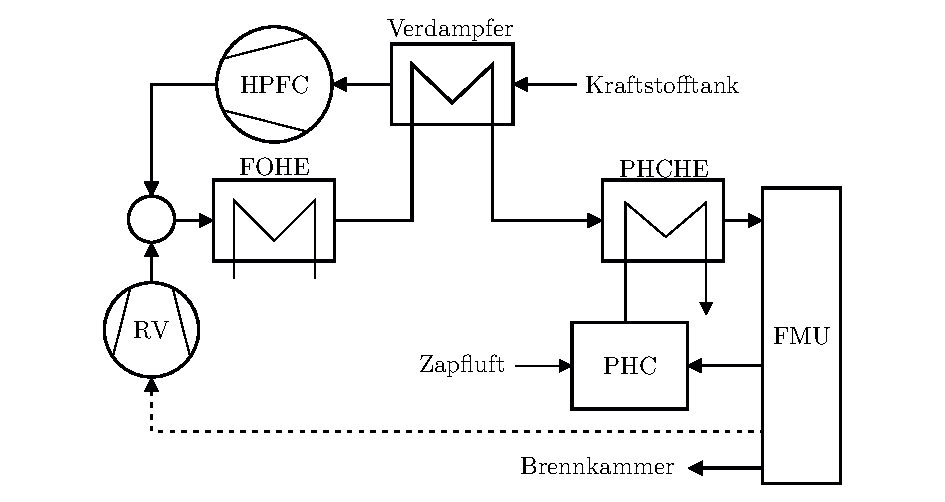
\includegraphics[width=1\linewidth]{4_Abbildungen/2_Hauptteil/Kraftstoffsystem Abbildungen/after.pdf}
  \caption{Wasserstoffkraftstoffsystem mit Verdichter und Verdampfer}
  \label{fig:verdampfer}
\end{figure}
\FloatBarrier 

Der Wasserstoff wird in dem Triebwerk zunächst in dem Verdampfer unter Zuführung des Wärmestroms $|\dot{Q}_\mathrm{V}|$ aus dem Hochdrucksystem gerade vollständig verdampft. Hierbei liegt über die Niederdruckseite des Wärmeübertragers das Druckverhältnis $\pi_{\mathrm{V,LP}}$ an. Der Hochdruckverdichter fördert den Wasserstoff mit dem Druck $p_{\mathrm{HPFC}}$ in das Hochdrucksystem, sodass der Brennkammer-Eintrittsdruck $p_{\mathrm{BK}}$ erreicht wird. Der Hochdruckverdichter arbeitet mit dem isentropen Wirkungsgrad $\eta_{\mathrm{HPFC}}$ und benötigt die Leistung $P_{\mathrm{HPFC}}$. 

Die Hochdruckseite gleicht dem Kraftstoffsystem mit Hochdruckpumpe mit dem einzigen Unterschied, dass zwischen den Wärmeübertragern mit dem Klima-/Ölsystem und dem Wärmeübertrager der parallelen Wasserstoffverbrennung die Hochdruckseite des Verdampfers durchlaufen wird. Hier wird die Wärme $\dot{Q}_\mathrm{V}$ an das Niederdrucksystem abgegeben und es liegt das Druckverhältnis $\pi_{\mathrm{V,HP}}$ an. Der Verdampfer wird auf der Hochdruckseite vor dem Wärmeübertrager mit der parallelen Wasserstoffverbrennung positioniert, um die maximale Wasserstofftemperatur zu mindern. Die geringere Maximaltemperatur ermöglicht eine geringere Abgastemperatur der parallelen Wasserstoffverbrennung und reduziert somit ihren Wasserstoffverbrauch.

\subsection{Architektur mit Vormischung}

Dieses Kraftstoffsystem zeichnet sich dadurch aus, dass an zwei unterschiedliche Positionen Kraftstoff von der Kraftstoffregeleinheit rezirkuliert wird. Zum einen wie auch bei den anderen Wasserstoff-Kraftstoffsystemen über einen Rezirkulationsverdichter hinter den Hochdruckverdichter. Ein kleiner rezirkulierter Kraftstoffmassenstrom $\dot{m}_\mathrm{V}$ wird stattdessen gedrosselt und vor den Hochdruckverdichter rezirkuliert, um den aus dem Kraftstofftank geförderten Wasserstoff ohne den Einsatz zusätzlicher Wärmeübertrager zu verdampfen. Das Hochdrucksystem ist identisch zu dem Hochdrucksystem des Kraftstoffsystems mit Hochdruckpumpe (Siehe Abbildung \ref{fig:vormischung}).

\begin{figure}[ht]
\centering
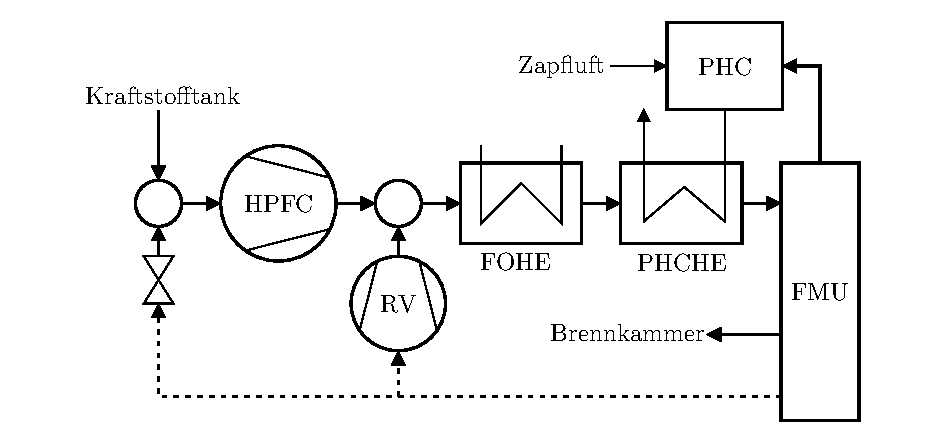
\includegraphics[width=1\linewidth]{4_Abbildungen/2_Hauptteil/Kraftstoffsystem Abbildungen/dual.pdf}
  \caption{Wasserstoffkraftstoffsystem mit Verdichter und Vormischung}
  \label{fig:vormischung}
\end{figure}
\FloatBarrier 

\subsection{Variablen und Parameter}

Die abhängigen Variablen der Modellierungen der Wasserstoff-Kraftstoffsysteme sind der Brennkammer-Eintrittsdruck $p_{\mathrm{BK}}$, die Brennkammer-Eintrittstemperatur $T_\mathrm{BK}$ und die Wärmeübertrager-Eintrittstemperatur $T_\mathrm{W}$. Die Parameter und unabhängigen Variablen der Modellierungen sind in Tabelle \ref{Tab:h2_params} zusammengefasst.

\begin{table}[ht]
    \centering
	\caption{Variablen der Modellierungen der Wasserstoff-Kraftstoffsysteme}
	\begin{tabular} {|l|c|l|c|} \hline%
    \multicolumn{4}{|c}{Alle Wasserstoff-Kraftstoffsysteme}\\ \hline
    \multicolumn{2}{|c}{Parameter} & \multicolumn{2}{|c|}{unabhängige Variablen}\\ \hline\hline%
    isentroper Wirkungsgrad RV & $\eta_\mathrm{RV}$ & RV-Leistung & $P_{\mathrm{RV}}$ \\ \hline
    Kraftstoff-Eintrittsdruck & $p_0$ & rezirkulierter Massenstrom & $\dot{m}_\mathrm{R}$ \\ \hline
    Kraftstoff-Eintrittstemperatur & $T_0$ & Enthalpie des rezirkulierten H$_2$ & $h_\mathrm{R}$ \\ \hline
    PHCHE-Druckverhältnis  & $\pi_{\mathrm{PHC}}$ & Druck des rezirkulierten H$_2$ & $p_\mathrm{R}$\\ \hline
    FOHE-Wärme & $\dot{Q}_{\mathrm{FOHE}}$ & PHCHE-Wärme  & $\dot{Q}_{\mathrm{PHC}}$\\ \hline
    FOHE-Druckverhältnis & $\pi_{\mathrm{FOHE}}$ & \multicolumn{2}{c|}{}\\ \hline
    Brennkammer-Massenstrom & $\dot{m}_{\mathrm{BK},0}$ & \multicolumn{2}{c|}{}\\ \hline
    Leitungs-Druckverluste & $\Delta p_{\mathrm{L}}$ & \multicolumn{2}{c|}{}\\ \hline
    Injektor-Druckverluste & $\Delta p_{\mathrm{inj}}$ & \multicolumn{2}{c|}{}\\ \hline\hline
	\multicolumn{4}{|c|}{Architektur mit Hochdruckpumpe}\\ \hline
    \multicolumn{2}{|c}{Parameter} & \multicolumn{2}{|c|}{unabhängige Variablen}\\ \hline\hline%
    isentroper Wirkungsgrad HPFP & $\eta_{\mathrm{HPFP}}$ & HPFP-Austrittsdruck & $p_{\mathrm{HPFP}}$ \\ \hline
    & & HPFP-Leistung & $P_{\mathrm{HPFP}}$ \\ \hline\hline
    \multicolumn{4}{|c|}{Architektur mit Verdampfer}\\ \hline
    \multicolumn{2}{|c}{Parameter} & \multicolumn{2}{|c|}{unabhängige Variablen}\\ \hline\hline%
    isentroper Wirkungsgrad HPFC & $\eta_{\mathrm{HPFC}}$ & HPFC-Austrittsdruck & $p_{\mathrm{HPFC}}$ \\ \hline
    Druckverhältnis LP-Verdampfer & $\pi_{\mathrm{V,LP}}$ & HPFC-Leistung & $P_{\mathrm{HPFC}}$ \\ \hline
    Druckverhältnis HP-Verdampfer & $\pi_\mathrm{V,HP}$ & Verdampfer-Wärme & $|\dot{Q}_\mathrm{V}|$ \\ \hline\hline
    \multicolumn{4}{|c|}{Architektur mit Vormischung}\\ \hline
    \multicolumn{2}{|c}{Parameter} & \multicolumn{2}{|c|}{unabhängige Variablen}\\ \hline\hline%
    isentroper Wirkungsgrad HPFC & $\eta_{\mathrm{HPFC}}$ & HPFC-Austrittsdruck & $p_{\mathrm{HPFC}}$ \\ \hline
    \multicolumn{2}{|c|}{}& HPFC-Leistung & $P_{\mathrm{HPFC}}$ \\ \hline
    \multicolumn{2}{|c|}{}& Massenstrom Verdampfung & $\dot{m}_\mathrm{V}$ \\ \hline
    \end{tabular}	
    \label{Tab:h2_params}%
\end{table}
\FloatBarrier 

\section{Modellierung der Komponenten}

Im Folgenden werden die Modellierungen der verschiedenen Komponenten erläutert, die in den Kraftstoffsystemen zum Einsatz kommen. Neben Modellen für Verdichter und Pumpen wird ein Modell für die Wärmeübertrager benötigt. Für die Modellierung der Wasserstoff-Kraftstoffsysteme ist zusätzlich ein Modell für die parallele Wasserstoffverbrennung erforderlich. Darüber hinaus werden die Korrektur des Kraftstoffmassenstroms in Abhängigkeit von der Brennkammereintrittstemperatur sowie für die Hochdruckwellen-Leistungsentnahme beschrieben.

\subsection{Pumpen und Verdichter}

Sämtliche Verdichter- und Pumpentypen werden durch die Definition des isentropen Wirkungsgrad $\eta_s$

\begin{equation}\label{Eq:isentropic}
	\eta_s=\frac{h_2-h_1}{h_{2,s}-h_1}
\end{equation}

modelliert. Dabei werden neben dem isentropen Wirkungsgrad auch der Austrittsdruck $p_2$, der Eintrittsdruck $p_1$, die Eintrittstemperatur $T_1$ und somit die spezifische Eintrittsenthalpie $h_1(T_1, p_1)$ sowie die spezifische Eintrittsentropie $s_1(T_1, p_1)$ als bekannt vorausgesetzt. Die Austrittstemperatur des reversiblen Prozesses $T_{2,s}$ kann iterativ mit der spezifischen Eintrittsentropie $s_1$ und dem Austrittsdruck $p_2$ bestimmt werden. $T_{2,s}$ wird mit der Zustandsgleichung für ideale Gase/Flüssigkeiten unter Annahme einer konstanten spezifischen isobaren Wärmekapazität $c_p$ abgeschätzt. Die Formel für die Differenz der spezifischen Entropie $s(p,T_2)-s(p, T_1)$

\begin{equation}\label{Eq:entropy}
	s(T_2,p)-s(T_1, p)=\cancel{s(T_0,p_0) - s(T_0,p_0)} + c_p(T_1,p) ln\left(\frac{T_2}{T_1}\right) - {\cancel{\overbrace{R ln\frac{p}{p}}^{\substack{\text{Nur bei } \\ \text{idealem Gas}}}}}
\end{equation}

eines ideales Fluids mit zwei unterschiedlichen Temperaturen wird umgestellt, um einen Schätzwert für die Austrittstemperatur des reversiblen Prozesses $T_{2,s}^{n+1}$

\begin{equation}\label{Eq:entropy-temperature}
	T_{2,s}^{n+1}=T_{2,s}^n\mathrm{exp}\left(\frac{s(T_1, p_1)-s(T_{2,s}^n, p_2)}{c_p(T_1, p_1)}\right)
\end{equation}

zu berechnen. Aus der iterativ berechneten Austrittstemperatur ergibt sich die spezifische Austrittsenthalpie $h_{2,s}$ des reversiblen Prozesses und aus Gleichung \ref{Eq:isentropic} folgt direkt die spezifische Austrittsenthalpie des realen Prozesses $h_2$. Anschließend wird mit der spezifischen Austrittsenthalpie und dem Austrittsdruck $p_2$ iterativ die Austrittstemperatur des realen Prozesses $T_2$ bestimmt. Die Formel für die Differenz der spezifischen Enthalpie $h(T_2,p)-h(T_1,p)$

\begin{equation}\label{Eq:enthalpy}
	h(T_2,p)-h(T_1,p)=\cancel{h(T_0,p_0) - h(T_0,p_0)} + c_p(T_1,p)(T_2 - T_1) - {\cancel{\overbrace{v(p-p)}^{\substack{\text{Nur bei idealer} \\ \text{Flüssigkeit}}}}}
\end{equation}

eines ideales Fluids mit zwei unterschiedlichen Temperaturen wird umgestellt, um einen Schätzwert für die Austrittstemperatur des realen Prozesses $T_2^{n+1}$

\begin{equation}\label{Eq:enthalpy-temperature}
	T_2^{n+1}=T_2^n+\frac{h_2-h(T_2^n,p_2)}{c_p(T_2^n,p_2)}
\end{equation}

zu berechnen. Abschließend wird die Verdichter-/Pumpenleistung $P$ 

\begin{equation}\label{Eq:power}
	P=\dot{m}(h_2-h_1)
\end{equation}

für den Kraftstoffmassenstrom $\dot{m}$ über die Energiebilanz um die Komponente bestimmt.

\subsection{Wärmeübertrager}

Da für die Zwecke dieser Modellierung ein stationärer Prozess im Designpunkt des Triebwerks angenommen wird, ist eine ausführliche Modellierung des Wärmeübergangs nicht notwendig. Eine Auslegungsrechnung der Wärmeübertrager wird in dieser Arbeit nicht angestrebt. Die einzige Erfordernis ist, dass die Wärmequelle der Wärmeübertrager in jedem Schnitt ein höheres Temperaturniveau als der Kraftstoffmassenstrom aufweist. Anhand des $\dot{H}-T$ Diagramms (Beispiel siehe Abbildung \ref{fig:hx}) kann festgestellt werden, ob über den gesamten Wärmeübertrager eine minimale Temperaturdifferenz $\Delta T_{min}$ zwischen Wärmequelle und Kraftstoffstrom eingehalten werden kann.


\begin{figure}[ht]
\centering
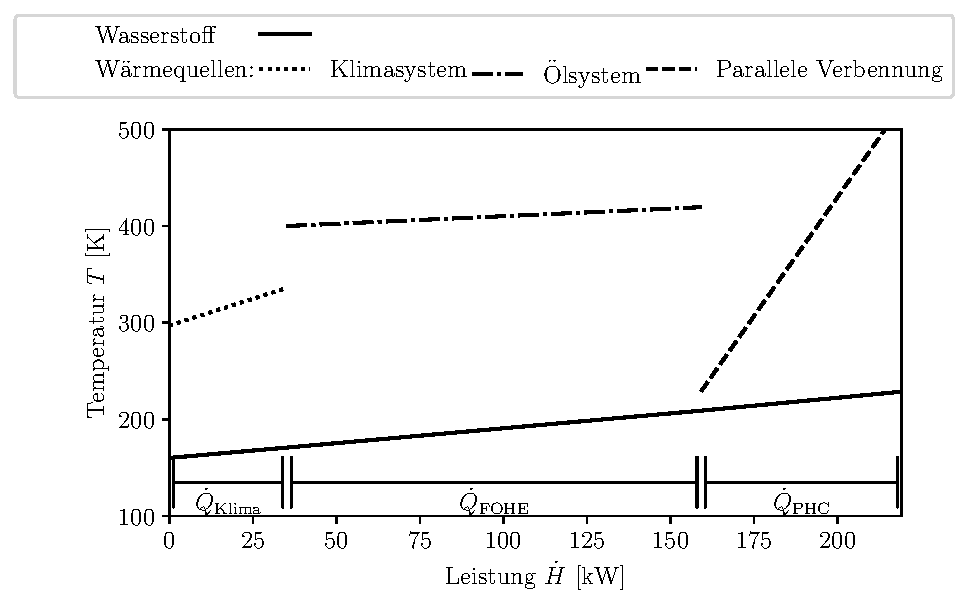
\includegraphics[width=1\linewidth]{4_Abbildungen/2_Hauptteil/hx.pdf}
  \caption{Wärmestromdiagramm für ein Wasserstoffkraftstoffsystem}
  \label{fig:hx}
\end{figure}
\FloatBarrier 

 Aus dem Eintrittszustand des Kraftstoffs in den Wärmeübertrager $T_1, p_1$ ergibt sich die spezifische Enthalpie des Kraftstoff im Eintritt in den Wärmeübertrager $h_1$. Die spezifische Austrittsenthalpie $h_2$

\begin{equation}\label{Eq:energy-hx}
	h_2=h_1 +q=h_1+\frac{\dot{Q}}{\dot{m}}
\end{equation}

erschließt sich direkt aus der Energiebilanz um die Kraftstoffseite des Wärmeübertragers mit dem Wärmestrom $\dot{Q}$ und dem Kraftstoffmassenstrom $\dot{m}$. Über den Wärmeübertrager besteht infolge von Strömungsverlusten ein Druckverhältnis $\pi$. Der Austrittsdruck $p_2$

\begin{equation}\label{Eq:pressuredrop}
	p_2 = p_1 \pi
\end{equation}

fällt somit geringer als der Eintrittsdruck aus. Für die Zwecke dieser Arbeit stellt das Druckverhältnis eine Auslegungsgröße dar und wird daher im Betriebspunkt als konstanten Wert angenommen. Abschließend wird Gleichung \ref{Eq:enthalpy-temperature} erneut eingesetzt, um iterativ die Austrittstemperatur $T_2$ des Kraftstoffs aus dem Wärmeübertrager zu bestimmen.

\subsection{Kraftstoffmischung}

In der Kraftstoffmischung werden die Kraftstoffmassenströme $\dot{m}_{1,\mathrm{\rom{1}}}$ und $\dot{m}_{1,\mathrm{\rom{2}}}$, mit demselben Eintrittsdruck $p_1$, aber unterschiedlichen Eintrittsenthalpien $h_{1,\mathrm{\rom{1}}}, h_{1,\mathrm{\rom{2}}}$ miteinander vermischt. Der Austrittsmassenstrom $\dot{m}_2$

\begin{equation}\label{Eq:mass}
	\dot{m}_2 = \dot{m}_{1,\mathrm{\rom{1}}}+\dot{m}_{1,\mathrm{\rom{2}}}
\end{equation}

berechnet sich aus der Massenbilanz um die Mischung. Die Austrittsenthalpie der Kraftstoffmischung 

\begin{equation}\label{Eq:energy-mix}
	h_{2} = \frac{\dot{m}_{1,\mathrm{\rom{1}}}h_{1,\mathrm{\rom{1}}}+\dot{m}_{1,\mathrm{\rom{2}}}h_{1,\mathrm{\rom{2}}}}{\dot{m}_2}
\end{equation}

wird mit der Energiebilanz um die Mischung bestimmt.  Druckverluste in der Mischung werden vernachlässigt, somit entspricht der Austrittsdruck $p_2$, dem Eintrittsdruck $p_1$. Abschließend wird Gleichung \ref{Eq:enthalpy-temperature} erneut eingesetzt, um iterativ die Austrittstemperatur $T_2$ des gemischten Kraftstoffmassenstroms zu bestimmen. 

\subsection{Parallele Wasserstoffverbrennung}

In den Wasserstoff-Kraftstoffsystemen ist nicht ausreichend Abwärme vorhanden, um den Wasserstoff auf beliebige Brennkammer-Eintrittstemperatur zu erwärmen. In dieser Arbeit wird der zusätzlicher Wärmebedarf durch parallele Wasserstoffverbrennung in einer separaten Brennkammer aufgebracht. Die Brennkammer wird mit Wasserstoff von der Kraftstoffregeleinheit und mit Fan-Zapfluft versorgt. Ziel der Modellierung der parallelen Wasserstoffverbrennung ist es, diesen Mehrbedarf an Wasserstoff und die erforderliche Leistung für die Bereitstellung der Zapfluft zu berechnen. Für diese Betrachtung wird Zapfluft als eine Mischung der idealen Gase Sauerstoff und Stickstoff, mit den spezifischen isobaren Wärmekapazitäten $c_{p,\mathrm{O}_2}, c_{p,\mathrm{N}_2}$ modelliert. Wasserstoff und das durch die Verbrennung erzeugte Wasser werden ebenfalls als ideale Gase mit den Wärmekapazitäten $c_{p,\mathrm{H}_2}, c_{p,\mathrm{H}_2\mathrm{O}}$ modelliert. Zunächst wird das stöchiometrische Sauerstoff/Wasserstoffmassenverhältnis $\frac{\dot{m}_{\mathrm{O}_2, \mathrm{st}}}{\dot{m}_{\mathrm{H}_2,\mathrm{st}}}$ 

\begin{equation}\label{Eq:stoichometric}
	\frac{\dot{m}_{\mathrm{O}_2,\mathrm{st}}}{\dot{m}_{\mathrm{H}_2,\mathrm{st}}}=\frac{M_{R,\mathrm{O}_2}}{2M_{R,\mathrm{H}_2}}
\end{equation}

mit den molaren Massen $M_{R,\mathrm{O}_2}$ und $M_{R,\mathrm{H}_2}$ berechnet. Mit dem Kraftstoff-Luft-Äquivalenz-verhältnis $\phi_{\mathrm{PHC}}$ wird der unverbrannte Sauerstoffmassenstrom $\dot{m}_{\mathrm{B},\mathrm{O}_2}$ 

\begin{equation}\label{Eq:oxygen}
	\frac{\dot{m}_{B,O_2}}{\dot{m}_{H_2}}=\frac{M_{R,O_2}}{2M_{R,H_2}}\left(\frac{1}{\phi_{PHC}}-1\right)
\end{equation}

im Verhältnis zum Wasserstoffmassenstrom $\dot{m}_{\mathrm{H}_2}$ berechnet. Mit dem Sauerstoffmassenanteil in Luft $w_{\mathrm{L, O}_2}$ wird aus Gleichungen \ref{Eq:stoichometric} und \ref{Eq:oxygen} eine Gleichung für den Stickstoffmassenstrom $\dot{m}_{\mathrm{N}_2}$ 

\begin{equation}\label{Eq:nitrogen}
	\frac{\dot{m}_{\mathrm{N}_2}}{\dot{m}_{\mathrm{H}_2}}=\frac{M_{R,\mathrm{O}_2}}{2M_{R,\mathrm{H}_2}}\frac{1-w_{\mathrm{L,O}_2}}{\phi_{\mathrm{PHC}}w_{\mathrm{L,O}_2}}
\end{equation}

im Verhältnis zum Wasserstoffmassenstrom hergeleitet. Nun wird mit der molaren Masse von Wasser $M_{R, \mathrm{H}_2\mathrm{O}}$ die Masse an durch die Verbrennung produziertem Wasser $\dot{m}_{\mathrm{H}_2\mathrm{O}}$

\begin{equation}\label{Eq:water}
	\frac{\dot{m}_{\mathrm{H}_2\mathrm{O}}}{\dot{m}_{\mathrm{H}_2}}=\frac{M_{R,\mathrm{H}_2\mathrm{O}}}{M_{R,\mathrm{H}_2}}
\end{equation}

im Verhältnis zum Wasserstoffmassenstrom berechnet. Anschließend wird die Energiebilanz für die parallele Brennkammer und die Abgasseite des nachgeschalteten Wärmeübertragers aufgestellt. Dabei wird die im Wärmeübertrager abgegebene Wärme $\dot{Q}_{\mathrm{PHC}}$

\begin{equation}\label{Eq:energy-phc}
\begin{multlined}
	\dot{Q}_{\mathrm{PHC}}=(\dot{m}_{\mathrm{N}_2}c_{p,\mathrm{N}_2}+\dot{m}_{\mathrm{B,O}_2}c_{p,\mathrm{O}_2})(T_\mathrm{Z}-T_\mathrm{B})+\dot{m}_{\mathrm{O}_2,\mathrm{st}}\frac{\dot{m}_{\mathrm{H}_2}}{\dot{m}_{\mathrm{H}_2,\mathrm{st}}}c_{p,\mathrm{O}_2}(T_\mathrm{Z}-T_{\mathrm{ref}}) \\
    +\dot{m}_{\mathrm{H}_2}(c_{p,\mathrm{H}_2}(T_{\mathrm{BK}}-T_{\mathrm{ref}})+H_{u,\mathrm{H}_2})-\dot{m}_{\mathrm{H}_2\mathrm{O}}c_{p,\mathrm{H}_2\mathrm{O}}(T_{\mathrm{B}}-T_{\mathrm{ref}})
\end{multlined}
\end{equation}

sowie der untere Heizwert von Wasserstoff $H_{u, \mathrm{H}_2}$ bei der Referenztemperatur $T_{\mathrm{ref}}$ berücksichtigt. Die Eintrittstemperatur der Zapfluft $T_\mathrm{Z}$ wird als bekannt vorausgesetzt, und es wird eine vollständige Verbrennung mit einem Wirkungsgrad von $100\,\%$ angenommen. Die Temperatur der abgekühlten Abgase $T_\mathrm{B}$  

\begin{equation}\label{Eq:deltat}
	T_\mathrm{B} = T_{\mathrm{H}_2}+\Delta T_\mathrm{PHC}
\end{equation}

wird aus der Eintrittstemperatur des kalten Wasserstoffs in den Wärmeübertrager $T_{\mathrm{H}_2}$ und der Temperaturdifferenz $\Delta T_{\mathrm{PHC}}$ berechnet. Um den Wasserstoffbedarf $\dot{m}_{\mathrm{PHC}}$ zu ermitteln, wird die Energiebilanz durch den Wasserstoffmassenstrom geteilt und nach dem Wasserstoffmassenstrom umgestellt

\begin{equation}\label{Eq:phc}
	\dot{m}_{\mathrm{PHC}}=\frac{\dot{Q}_{\mathrm{PHC}}}{
    \begin{aligned}
    \left(\frac{\dot{m}_{\mathrm{N}_2}}{\dot{m}_{\mathrm{H}_2}}c_{p,\mathrm{N}_2}+\frac{\dot{m}_{\mathrm{B,O}_2}}{\dot{m}_{\mathrm{H}_2}}c_{p,\mathrm{O}_2}\right)(T_\mathrm{Z}-T_\mathrm{B})+\frac{\dot{m}_{\mathrm{O}_2,\mathrm{st}}}{\dot{m}_{\mathrm{H}_2,\mathrm{st}}}c_{p,\mathrm{O}_2}(T_\mathrm{Z}-T_{\mathrm{ref}})\\
    +c_{p,\mathrm{H}_2}(T_{\mathrm{BK}}-T_{\mathrm{ref}})-\frac{\dot{m}_{\mathrm{H}_2\mathrm{O}}}{\dot{m}_{\mathrm{H}_2}}c_{p,\mathrm{H}_2\mathrm{O}}(T_\mathrm{B}-T_{\mathrm{ref}})
    \end{aligned}
    }\,.
\end{equation}

Abschließend wird die infolge der Fan-Zapfluftentnahme erforderliche zusätzliche Niederdruckwellen-Leistung $P_\mathrm{Z}$

\begin{equation}\label{Eq:fanpower}
	P_\mathrm{Z} = \frac{\dot{m}_{\mathrm{PHC}}}{\eta_1}\left(\frac{\dot{m}_\mathrm{{N}_2}}{\dot{m}_{\mathrm{H}_2}}c_{p,\mathrm{N}_2}+\left(\frac{\dot{m}_{\mathrm{B,O}_2}}{\dot{m}_{\mathrm{H}_2}}+\frac{\dot{m}_{\mathrm{O}_2,\mathrm{st}}}{\dot{m}_{\mathrm{H}_2,\mathrm{st}}}\right)c_{p,\mathrm{O}_2}\right)(T_\mathrm{Z}-T_\mathrm{U})
\end{equation}

mit der Umgebungstemperatur $T_\mathrm{U}$ und dem mechanischen Wirkungsgrad der Niederdruckwelle $\eta_1$ berechnet. Die Modellierung der parallelen Wasserstoffverbrennung erfordert die in Tabelle \ref{Tab:phc_params} aufgeführten Parameter.

\begin{table}[ht]
    \centering
	\caption{Parameter der Modellierung der parallelen Wasserstoffverbrennung}
	\begin{tabular} {|l|c|} \hline%
    \multicolumn{2}{|c|}{Parameter} \\ \hline\hline
    spezifische isobare Wärmekapazität Sauerstoff & $c_{p, O_2}$ \\ \hline
    spezifische isobare Wärmekapazität Stickstoff & $c_{p, N_2}$ \\ \hline
    spezifische isobare Wärmekapazität Wasserstoff & $c_{p, H_2}$ \\ \hline
    spezifische isobare Wärmekapazität Wasser & $c_{p, \mathrm{H}_2\mathrm{O}}$ \\ \hline
    molare Masse Sauerstoff & $M_{R, \mathrm{O}_2}$ \\ \hline
    molare Masse Wasserstoff & $M_{R, \mathrm{H}_2}$ \\ \hline
    molare Masse Wasser & $M_{R, \mathrm{H}_2\mathrm{O}}$ \\ \hline
    Äquivalenzverhältnis & $\phi_{\mathrm{PHC}}$ \\ \hline
    Sauerstoffmassenanteil & $w_{\mathrm{L,O}_2}$ \\ \hline
    unterer Heizwert Wasserstoff & $H_{u, \mathrm{H}_2}$ \\ \hline
    Referenztemperatur & $T_{\mathrm{ref}}$ \\ \hline
    Zapflufttemperatur & $T_\mathrm{Z}$ \\ \hline
    Umgebungstemperatur & $T_\mathrm{U}$ \\ \hline
    Wirkungsgrad Niederdruckwelle & $\eta_1$ \\ \hline
    Wärmeübertrager Temperaturdifferenz & $\Delta T_{\mathrm{PHC}}$ \\ \hline  
    
	\end{tabular}	
    \label{Tab:phc_params}%
\end{table}
\FloatBarrier 

\subsection{Korrektur des Kraftstoffmassenstroms}

Die Kraftstoffmassenströme $\dot{m}_{\mathrm{BK},0}$ im Reiseflug gelten für Referenz-Kraftstofftemperaturen $T_{\mathrm{ref,H_2}}$ beziehungsweise $T_{\mathrm{ref, Jet-A}}$. Der erforderliche Kraftstoffmassenstrom $\dot{m}_{BK}$

\begin{equation}\label{Eq:tempcorr}
	\dot{m}_{\mathrm{BK}}=\dot{m}_{\mathrm{BK},0}\frac{H_{u,\mathrm{k}}}{H_{u,\mathrm{k}}+h_\mathrm{k}(T_{\mathrm{BK}}, p_{\mathrm{BK}})-h_\mathrm{k}(T_{\mathrm{ref,k}}, p_{\mathrm{BK}})}
\end{equation}

wird entsprechend der tatsächlichen Brennkammereintrittstemperatur des Kraftstoffs mithilfe der jeweiligen Stoffmodelle korrigiert. Veränderungen in der Abgaszusammensetzung des Kreisprozesses werden vernachlässigt.

Um eine Vergleichbarkeit zwischen den Leistungs- und Wärmebedarfen zu ermöglichen, werden die Bedarfe in den zusätzlichen parasitären Kraftstoffverbrauch der jeweiligen Systeme umgerechnet. Der zusätzliche Kraftstoffverbrauch der Wärmebereitstellung ist durch die Modellierung der parallelen Wasserstoffverbrennung bereits berücksichtigt. Der zusätzliche Kraftstoffbedarf infolge der Leistungsentnahme von den Triebwerkswellen $\dot{m}_{BK,P}$

\begin{equation}\label{Eq:powerofftake}
	\dot{m}_{\mathrm{BK,P}}=\frac{P}{\eta_\mathrm{P}\left(H_{u,\mathrm{k}}+h_\mathrm{k}(T_{\mathrm{BK}}, p_{\mathrm{BK}})-h_\mathrm{k}(T_{\mathrm{ref,k}}, p_{\mathrm{BK}})\right)}
\end{equation}

 wird mit einem Ansatz von Scholz et al. \cite{Scholz.2013} berechnet. Hierfür wird der Wirkungsgrad $\eta_\mathrm{P}$ angenommen. Der gesamte geförderte Kraftstoffmassenstrom beträgt somit
 
 \begin{equation}\label{Eq:sum}
	\dot{m}_{\mathrm{k}}=\dot{m}_{\mathrm{BK}}+\dot{m}_{\mathrm{BK,P}}+\overbrace{\dot{m}_{\mathrm{PHC}}}^{\text{nur H}_2}
\end{equation}
 
 Die zusätzlichen erforderlichen Parameter sind in Tabelle \ref{Tab:fuel_corr_params} zusammengefasst.

 \begin{table}[ht]
    \centering
	\caption{Parameter für die Korrektur des Kraftstoffmassenstroms}
	\begin{tabular} {|l|c|} \hline%
    \multicolumn{2}{|c|}{Parameter} \\ \hline\hline
    unterer Heizwert H$_2$ & $H_{u,\mathrm{H}_2}$ \\ \hline
    unterer Heizwert Jet-A & $H_{u,\mathrm{Jet-A}}$ \\ \hline
    Referenztemperatur H$_2$ & $T_{\mathrm{ref, H}_2}$ \\ \hline
    Referenztemperatur Jet-A & $T_{\mathrm{ref, Jet-A}}$ \\ \hline
    Wirkungsgrad Leistungsentnahme & $\eta_\mathrm{P}$ \\ \hline    
	\end{tabular}	
    \label{Tab:fuel_corr_params}%
\end{table}
\FloatBarrier 

\section{Stoffmodelle}

Für die Modellierung der Kraftstoffsysteme sind Stoffmodelle erforderlich, um thermodynamische Zustandsgrößen wie spezifische Enthalpie und Entropie in Abhängigkeit von Temperatur und Druck der Kraftstoffe bestimmen zu können. In diesem Abschnitt werden die für Kerosin und Wasserstoff verwendeten Stoffmodelle erläutert.

\subsection{Wasserstoff Stoffmodell}

Wasserstoff besteht aus zwei unterschiedlichen Kernspin-Isomeren, Parawasserstoff und Orthowasserstoff. Da sich die beiden Spin-Isomer in ihrer Wärmekapazität bei niedrigen Temperaturen stark unterscheiden, muss das Stoffmodell das Verhältnis der Kern-Isomer berücksichtigen. Bei Temperaturen oberhalb von \SI{200}{\K} liegen die Isomere im thermischen Gleichgewicht in einem Verhältnis von 3:1 zwischen Ortho- und Parawasserstoff vor. Flüssiger Wasserstoff besteht im Gleichgewichtszustand hingegen aus nahezu purem Parawasserstoff (Siehe Abbildung \ref{fig:spin}). In Abwesenheit eines Katalysators wird der Gleichgewichtszustand nur langsam erreicht. Daher ist davon auszugehen, dass der ursprünglich kryogen gelagerte Wasserstoff im Kraftstoffsystem nahezu vollständig in Form von Parawasserstoff vorliegt. Für die Parametrierung des Stoffmodells wird daher eine Zusammensetzung aus purem Parawasserstoff angenommen. \cite{Buntkowsky.2022}

\begin{figure}[ht]
\centering
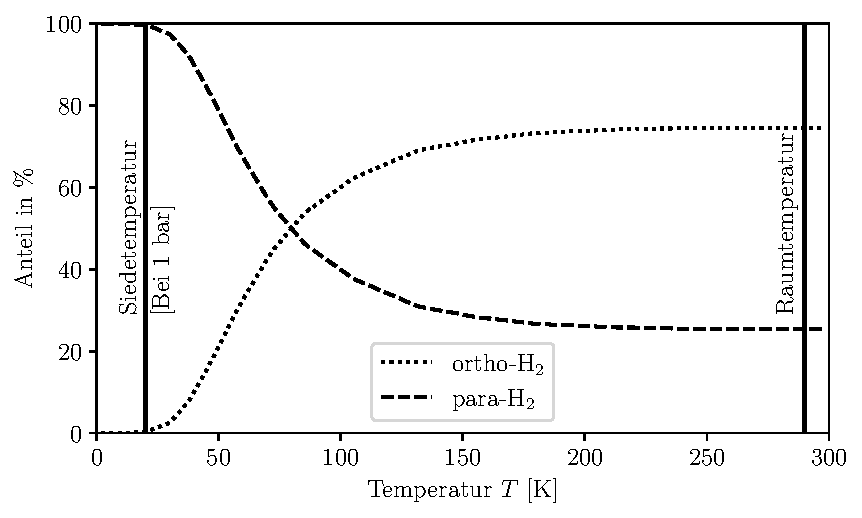
\includegraphics[width=1\linewidth]{4_Abbildungen/2_Hauptteil/spin.pdf}
  \caption{Wasserstoff Kernspin-Isomer Anteile nach \cite{Buntkowsky.2022}}
  \label{fig:spin}
\end{figure}
\FloatBarrier 

Für die Berechnung der thermodynamischen Zustandsgrößen von Parawasserstoff, wird ein am Institut für Strahlantriebe und Turbomaschinen (IST) entwickeltes Stoffmodell weiterentwickelt. Das Stoffmodell basiert auf einem von Leachman et al. \cite{Leachman.2017} beschriebenen Ansatz, der die Zustandsgrößen in Abhängigkeit der Helmholtz-Energie, die auch als freie Energie bekannt ist, setzt. Leachman et al. berechnen die entdimensionierte Helmholtz-Energie $\alpha$ 

\begin{equation}\label{Eq:free-energy}
    \alpha(\delta, \tau) = \alpha^0(\delta, \tau) + \alpha^r(\delta, \tau)
\end{equation}

als Summe der Idealgaskomponente $\alpha^0$ und des Anteils aufgrund von Kompressibilität $\alpha^r$. Hierbei gelten folgende Definitionen der entdimensionierten Helmholtz-Energie $\alpha$ und der entdimensionierten Variablen $\delta$ und $\tau$

\begin{equation}
    \alpha = \frac{a}{RT}, \delta = \frac{\rho}{\rho_c}, \tau = \frac{T_c}{T} \,.
\end{equation}

Mit einer semi-empirischen Zustandsgleichung berechnen Leachman et al die Idealgaskomponente der entdimensionierten freien Energie $\alpha^0$

\begin{equation}\label{Eq:free-energy-idealgas}
    \alpha^0(\tau,\delta)=ln(\delta)+(a_0-1)\mathrm{ln}(\tau)+a_1+a_2\tau-\sum_{i=3}^{m}a_i\frac{(\frac{T_c}{\tau})^{k_i}}{k_i(k_i+1)}+\sum_{i=m+1}^{n}a_i\mathrm{ln}\left(1-e^{\frac{-k_i\tau}{T_c}}\right) \,.
\end{equation}

Die Zustandsgleichung für den Anteil an der entdimensionierten freien Energie aufgrund von Kompressibilitätseffekten $\alpha^r$

\begin{equation}\label{Eq:free-energy-compressibility}
    \alpha^r(\tau,\delta)=\sum_{i=1}^{l}N_i\delta^{d_i}\tau^{t_i}+\sum_{i=l+1}^{m}N_i\delta^{d_i}\tau^{t_i}e^{-\delta^{p_i}}+\sum_{i=m+1}^{n}N_i\delta^{d_i}\tau^{t_i}e^{-\phi_i(\delta-D_i)^2-\beta_i(\tau-\gamma_i)^2)}
\end{equation}

orientiert sich an theoretischen und praktischen Abwägungen. Die in Gleichungen \ref{Eq:free-energy-idealgas} und \ref{Eq:free-energy-compressibility} enthaltenen Parameter werden durch Anpassung auf eine Datenbank experimenteller Daten bestimmt. Da die freie Energie eine Funktion von Dichte und Temperatur ist, der Zustand in dieser Arbeit hingegen in Form von Druck und Temperatur bekannt ist, wird die Dichte zunächst iterativ mithilfe des Newton-Raphson-Verfahrens bestimmt. Mit dem initialen Wert der Dichte $\rho_n$ wird ein Wert für den Druck $p_{\rho_n}$ 

\begin{equation}\label{Eq:pressure-guess}
    p_{\rho_n}=\rho_nRT\left(1+\delta_n\frac{\partial\alpha^r}{\partial\delta}|_{\delta_n, \tau}\right)
\end{equation}

geraten, wobei $\frac{\partial\alpha^r}{\partial\tau}$ mit Gleichung \ref{Eq:free-energy-compressibility} berechnet wird. Anschließend wird mit Gleichung \ref{Eq:pressure-guess} anhand von zwei Stützstellen ein Wert für die Änderungsrate des Drucks $\frac{\mathrm{d}p}{\mathrm{d}\rho}|_{\rho_n,\tau}$ zur Dichte bestimmt. Mithilfe des geratenen Drucks und der Änderungsrate wird der nächste Wert für die Dichte $\rho_{n+1}$

\begin{equation}\label{Eq:density_calc}
    \rho_{n+1}=\rho_n+\frac{p-p_{\rho_n}}{\frac{\mathrm{d}p}{\mathrm{d}\rho}|_{\rho_n,\tau}}
\end{equation}

berechnet. Mit Dichte und Temperatur beziehungsweise deren entdimensionierten Äquivalenten werden die freien Energien und die Ableitungen der freien Energien nach $\delta$ und $\tau$ berechnet. Diese Werte liefern die Grundlage für die Berechnung der notwendigen thermodynamischen Zustandsgrößen mit den in Tabelle \ref{Tab:thermodynamic_properties_h2} definierten Zustandsgleichungen.

\begin{table}[ht]
    \centering
	\caption{Formeln für thermodynamische Zustandsgrößen von Wasserstoff}
	\begin{tabular} {|l|c|c|} \hline%
		\multicolumn{2}{|c|}{Zustandsgröße}  & Formel\\ \hline\hline%
		  spezifische Enthalpie &$h$ 		  & $RT(\tau\frac{\partial\alpha}{\partial\tau}+\delta\frac{\partial\alpha^r}{\partial\delta}+1)$ \\ \hline%
		  spezifische Entropie& $s$ 		      &  $R(\tau\frac{\partial\alpha}{\partial\tau}-\alpha)$\\ \hline%
		spezifische isochore Wärmekapazität &$c_v$ 	    &  $-R\tau^2\frac{\partial^2\alpha}{\partial\tau^2}$\\ \hline%		
        spezifische isobare Wärmekapazität &$c_p$        &  $c_v+R\frac{\left(1+\delta\frac{\partial\alpha^r}{\partial\delta}-\delta\tau\frac{\partial^2\alpha^r}{\partial\delta\partial\tau}\right)^2}{1+2\delta\frac{\partial\alpha^r}{\partial\delta}+\delta^2\frac{\partial^2\alpha^r}{\partial\delta^2}}$\\ \hline%
	\end{tabular}	
    \label{Tab:thermodynamic_properties_h2}%
\end{table}
\FloatBarrier 

\subsection{Kerosin Stoffmodell}

Die Modellierung von Kerosin beziehungsweise Jet-A ist grundsätzlich mit Unsicherheit behaftet, da die Spezifikation des Kraftstoffs vergleichsweise große Abweichungen der Eigenschaften zulässt. Outcalt et al. \cite{Outcalt.2009} haben die Dichte von drei unterschiedlichen Proben an Jet-A Kraftstoff für Temperaturen zwischen \SI{270}{\K} und \SI{470}{\K} und Drücke zwischen \SI{83}{\kilo\Pa} und \SI{30}{\mega\Pa} gemessen und haben eine Abweichung von bis zu $4\,\%$ zwischen den Dichten der Proben ermittelt.

Da Kerosin kein Reinstoff, sondern eine Mischung von Kohlen-Wasserstoffverbindungen mit unterschiedlichen Kettenlängen ist, kann ein Kerosin Stoffmodell nicht mit demselben Ansatz wie das Wasserstoff Stoffmodell entwickelt werden. Stattdessen wird ein empirischer von McBridge et al. \cite{McBridge.2002} vorgeschlagenes Stoffmodell verwendet. Die Autoren haben generische empirische Formeln in Form von Polynomen für die Enthalpie, Entropie und isobare Wärmekapazität aufgestellt und anhand experimenteller Messungen der Zustandsgrößen für 2000 Spezies, inklusive Jet-A Kraftstoff, parametriert. Tabelle \ref{Tab:thermodynamic_properties_jeta} liefert einen Überblick über die verwendeten Zustandsgleichungen.

\begin{table}[ht]
    \centering
	\caption{Thermodynamische Zustandsgrößen von Jet-A Kraftstoff nach 
    \cite{McBridge.2002}}
	\begin{tabular} {|l|c|l|} \hline%
		\multicolumn{2}{|c|}{Zustandsgröße}  & Formel\\ \hline\hline%
		  spezifische Enthalpie &$h$ & $R(a_1T^{-2}+a_2T^{-1} +a_3$ \\ 
        & & $+a_4T+a_5T^2+a_6T^3+a_7T^4)$\\ \hline
		  spezifische Entropie& $s$ &  $R(-a_1T^{-1}+a_2ln(T)+a_3T$\\ 
        & & $+\frac{a_4T^2}{2}+\frac{a_5T^3}{3}+\frac{a_6T^4}{4}+\frac{a_7T^5}{5}+b_1)$\\ \hline
        spezifische isobare Wärmekapazität &$c_p$ &  $R(-\frac{a_1T^{-2}}{2}-a_2T^{-1}+a_3ln(T)+ a_4T$\\ 
	    & & $+\frac{a_5T^{2}}{2}+\frac{a_6T^{3}}{3}+\frac{a_7T^{4}}{4}+b_2)$\\ \hline
    \end{tabular}	
    \label{Tab:thermodynamic_properties_jeta}%
\end{table}
\FloatBarrier 

Da eine Berechnung der Dichte mit demselben Ansatz nicht möglich ist, werden in dieser Arbeit stattdessen die von Outcalt et al. \cite{Outcalt.2009} gemessenen Datenpunkte interpoliert beziehungsweise für Temperaturen unterhalb von \SI{270}{\K} extrapoliert. Als Datengrundlage wird die Probe Jet-A 4658 verwendet, da sie von den Autoren als die repräsentativste der Proben erachtet wird. Für die Berechnung der Dichte $\rho(T,p)$, werden die vier angrenzenden gemessenen Dichten $\rho(T_\mathrm{N},p_{\mathrm{N,n}})$, $\rho(T_\mathrm{N},p_{\mathrm{N,h}})$, $\rho(T_\mathrm{H},p_{\mathrm{H,n}})$ und $\rho(T_\mathrm{H},p_{\mathrm{H,h}})$ benötigt. Bei der Extrapolation werden stattdessen Messwerte der jeweils zwei nächsthöheren Temperaturen als Stützstellen verwendet. Da Outcalt et al. die Dichte für einheitliche Temperaturschritte, aber uneinheitliche Druckschritte gemessen haben, werden zunächst die Dichten $\rho(T_\mathrm{H}, p)$ und $\rho(T_\mathrm{N}, p)$ 

\begin{equation}\label{Eq:pressure-interp}
    \rho(T_i, p)= \rho(T_i, p_{i,\mathrm{n}}) + \frac{\rho(T_i, p_{i,\mathrm{h}})-\rho(T_i, p_{i,\mathrm{n}})}{p_{i,\mathrm{h}}-p_{i,\mathrm{n}}}(p-p_{i,\mathrm{n}}) 
\end{equation}

für den Druck interpoliert. Abschließend wird die Dichte $\rho(T,p)$

\begin{equation}\label{Eq:temperature-interp}
    \rho(T, p)= \rho(T_\mathrm{N}, p) + \frac{\rho(T_\mathrm{H}, p)-\rho(T_\mathrm{N}, p)}{T_\mathrm{H}-T_\mathrm{N}}(T-T_\mathrm{N}) 
\end{equation}

für die Temperatur interpoliert. 